\documentclass[10pt,twocolumn,letterpaper]{article}

\usepackage{icl_eee_cw}
\usepackage{times}
\usepackage{epsfig}
\usepackage{graphicx}
\usepackage{amsmath}
\usepackage{amssymb}
\usepackage{cite}
\usepackage{placeins}
\graphicspath{./assets}
% Include other packages here, before hyperref.

% If you comment hyperref and then uncomment it, you should delete
% egpaper.aux before re-running latex.  (Or just hit 'q' on the first latex
% run, let it finish, and you should be clear).
\usepackage[breaklinks=true,bookmarks=false]{hyperref}
\cvprfinalcopy%
\def\cvprPaperID{****} % *** Enter the CVPR Paper ID here
\def\httilde{\mbox{\tt\raisebox{-.5ex}{\symbol{126}}}}

% Pages are numbered in submission mode, and unnumbered in camera-ready
%\ifcvprfinal\pagestyle{empty}\fi
\setcounter{page}{1}
\begin{document}

%%%%%%%%% TITLE
\title{Max Wickham, mw1919, 01717673}
\maketitle
%\thispagestyle{empty}
%\vspace{-5cm}


%%%%%%%%% BODY TEXT
% \section{Tutorial 2 CNN Introduction}


% \paragraph{Task 1: Classification}
% % Figure~\ref{fig:1} shows a bar chart that presents the training and validation accuracy of several different design choices. The second test shown in the chart added an extra convolution layer with twice the convolutions as in the previous first layer, this increased both the training and test accuracy as it increased the model complexity, which was still low and so was underfitting to the data. Increasing the number of dense layers, again with twice the nodes oin the new first dense layer as before again increased both scores and didn't significantly change the generalisation error. This suggested that the model was still not complex enough. The 4th test introduced larger convolution sizes of 6 by 6 vs 3 by 3 in the second model and this also resulted in an increase in scores. Test 5 tries increasing the number of dense layers further relative to the 3rd test. This gives very little noticeable change which is interesting as even the generalisation error isn't affected suggesting this change did not increase the model complexity significantly. The final 2 tests try adding even more convolution layers which results in a higher training and validation accuracy than any other test but does increase generalisation error. The final test places the number of convolutions at each layer in increasing size which slightly reduces the results suggesting this is a worse strategy than placing them in increasing order. Figure~\ref{fig:2} shows the model used in the penultimate test which resulted in the highest validation score. Attempts at adding further convolution layers were unsuccessful at increasing this score as they resulted in too much overfitting.  

% Figure~\ref{fig:1} shows a bar chart that presents the training and validation accuracy of several different design choices. The second test added an extra convolution layer compared to the first test and this increased both the validation and training accuracy indicating underfitting was still present. Increasing the number of dense layers with twice the number of nodes as opposed to the old first dense layer again increased both scores and didn't significantly change the generalisation error. The fourth test increased the size of the convolutions to 6x6 vs 3x3 and this again increased the scores. The 5th test tries adding more dense layers relative to the third test but this causes little change, which was interesting as it didn't result in worse validation error suggesting greater overfitting hadn't occurred. The final two tests add even more convolution layers with the last test giving a worse score suggesting at this point the model was getting too complex. Figure~\ref{fig:2} shows the model used in the penultimate test which resulted in the highest validation score.



% \begin{figure}[ht]
%     \begin{center}
%         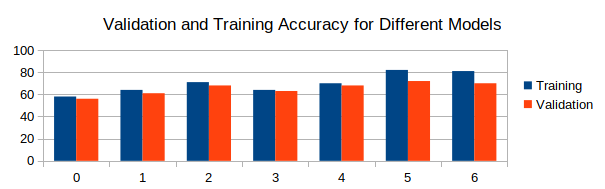
\includegraphics[width=1\linewidth]{assets/Part2Task1.png}
%         \caption{T1.1.1 Comparison of Training vs Validation Accuracy for Several Models}\label{fig:1}
%     \end{center}
% \end{figure}

% \begin{figure}[ht]
%     \begin{center}
%         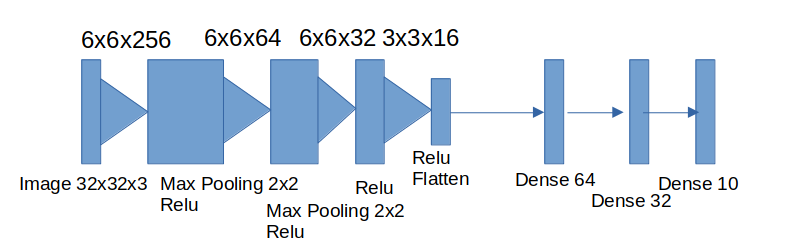
\includegraphics[width=1\linewidth]{assets/Part2Task12.png}
%         \caption{T1.1.2 Architecture of Most Successful Model}\label{fig:2}
%     \end{center}
% \end{figure}

% \paragraph{Task 2: Regression} The best model tried for this task is shown in Figure~\ref{fig:3}, and gave a minimum absolute percentage error of 52\% on the validation set. Figure~\ref{fig:4} shows the training and validation loss across different epochs for 3 models. Model 0 was the most successful on the validation set and decreasing the number of convolutions as in Model 1 resulted in a very similar training score but a worse validation score. Increasing the number of dense layers as in Model 2 gave a better training score but worse validation score suggesting that this increase resulted in overfitting. After about 25 epochs all three models had increasing validation loss which indicates that after this number of epochs they were begining to over-fit to the data set. Table~\ref{table:1} shows the minimum validation loss using the best model on the different faces of the house.

% \begin{figure}[ht]
%     \begin{center}
%         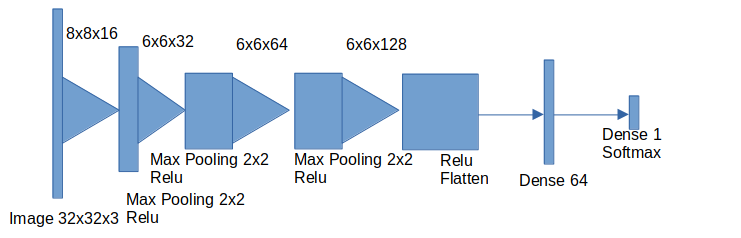
\includegraphics[width=1\linewidth]{assets/Part2Task21.png}
%         \caption{T1.2.1 Architecture of Most Successful Model}\label{fig:3}
%     \end{center}
% \end{figure}

% \begin{figure}[ht]
%     \begin{center}
%         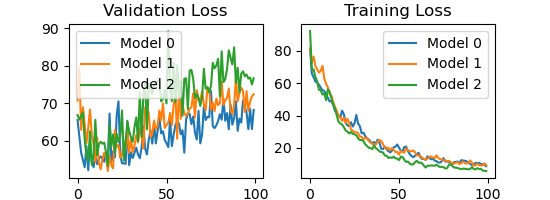
\includegraphics[width=1\linewidth]{assets/Part2Task2Front.png}
%         \caption{T1.2.1 Training and Validation loss, Front of the House}\label{fig:4}
%     \end{center}
% \end{figure}

% \begin{table}[ht]
%     \small
%     \centering
%     \begin{tabular}{|c|c|}
%         \hline
%         Face     & Validation Loss \\
%         \hline
%         Kitchen  & 52.2            \\
%         Bedroom  & 45.3            \\
%         Bathroom & 51.8            \\
%         \hline
%     \end{tabular}
%     \medbreak
%     \caption{T2.2 Validation loss for different house faces}
%     \label{table:1}
% \end{table}



% % When placing figures in \LaTeX, it's almost always best to use
% % \verb+\includegraphics+, and to specify the  figure width as a multiple of
% % the line width as in the example below
% % {\small\begin{verbatim}
% %    \usepackage[dvips]{graphicx} ...
% %    \includegraphics[width=0.8\linewidth]
% %                    {myfile.eps}
% % \end{verbatim}
% % }

\section{Tutorial 3 Network Training}

\paragraph{Task1: Tuning a Classification Model}
Figures~\ref{fig:t311},~\ref{fig:t312},~\ref{fig:t313} in the appendix show the validation and training accuracy and loss for each of the different augmentation strategies.
The soft strategy was a random translation with a height and width factor of 0.2 and a bilinear interpolation. Conversely, the aggressive strategy used was the same random translation accompanied with a random rotation of 0.2 and a random zoom with a height of 0.3. Table~\ref{table:t311} shows each strategies validation accuracy. \\
The soft augmentation strategy had the best result and the hard augmentation strategy gave the worst result. When looking at the loss curves for the three strategies it can be noted that only when using no augmentation does the validation loss start to increase with later epochs suggesting that overfitting is starting to occur at this point. In the other strategies, both of which use augmentation the loss is still decreasing by the last epoch suggestion that adding augmentation results in either more epochs or a more complex model needed to give overfitting due to the larger input space. This is good as it prevents the model from being too specific to the training data. \\
The poor performance of the hard augmentation may be due to the dataset being standardised at a similar zoom and rotation level meaning that this augmentation is forcing the model to be able to classify a much greater range of possible inputs requiring a more complex model or more epochs to get the same classification accuracy. \\
Batch normalisation was added after each of the max pooling payers following the convolution layers, dropout layers were added in the same place with a dropout value of 0.2 used. Dropout came first when using both. Table~\ref{table:t311} shows adding both batch normalisation and dropout was the most effective strategy. According to arXiv:1502.03167\cite{normalisation} batch normalisation prevents "small changes from being amplified into larger suboptimal changed" which can make the model more stable giving a higher accuracy. As said in the slides~\cite{slides3} dropout decreases overfitting so also increases accuracy in this case.
\\
Initialisation all the weights to zero gave an accuracy of exactly 10\%. This suggests that the input to the model has no effect on the output after training as the same number is always predicted. This is due to the zero values having no gradient so the weights aren't adjusted. 
\\
% Figure~\ref{fig:t34} shows the training and validation loss for each of the three SGD optimiser settings. As can be seen from the graph the validation loss of 0.0003 and 0.003 are very similar whilst 0.001 gives worse results. Both 0.003 and 0.001 have a loss the goes up then back down suggesting perhaps the learning rate is too big and they significantly miss a minimum.
% REDO GRAPH
% SGD IN TABLE?
% ADD ADAM
% Figure~\ref{fig:t34} shows the loss for each of the learning rates. The final validation loss seems to be lower the smaller the learning rate used which suggests that the larger learning rates are too big and may miss local minima causing the loss function to require more steps to reach a minimum due to oscillating either side of it. The smallest training step has a greater loss at first due to a less rapid approach to the minimum but once near the minimum it can approach it more accurately giving a lower loss in less time.
Figure~\ref{fig:t34} shows the loss for each of the learning rates. The larger the learning rate used the faster the loss decreases which is due to greater steps being taken along the gradient to reduce the loss \cite{slides3}. None of the three strategies used have any sign of overfitting with the validation loss always being very close to the training loss for a given learning rate. In this case the best learning rate tried is $0.003$.


\begin{table}[ht]
    \small
    \centering
    \begin{tabular}{|c|c|}
        \hline
        Strategy     & Validation Accuracy \\
        \hline
        No Augmentation  & 78\%           \\
        Soft Augmentation  & 82\%            \\
        Hard Augmentation & 73\%           \\
        Dropout & 82\% \\
        Batch Normalisation & 80 \% \\
        Batch Normalisation and Dropout & 84\% \\
        Zero Weight Initialisation & 10.000\% \\
        \hline
    \end{tabular}
    \medbreak
    \caption{T3.1 Validation accuracy for different models strategies}
    \vspace{-0.7cm}
    \label{table:t311}
\end{table}

\begin{figure}[ht]
    \begin{center}
        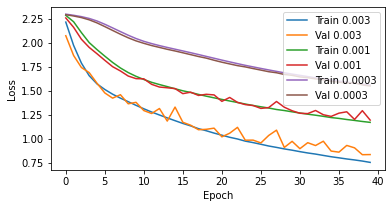
\includegraphics[width=1\linewidth]{/Part3.assets/sgd.png}
        \caption{T3.1.4 Validation and Training Loss For Different Learning Rates}
        \vspace{-0.7cm}
        \label{fig:t34}
    \end{center}
\end{figure}

%//TODO REDO This table

\section{Tutorial 4 Introduction to Common Neural Network Architectures}

\paragraph{Task1: Classification on Tiny Image Net}

% - training and validation accuracy curves for 
%     - vgg trainined from scratch
%     - pre trainined
%     - fine tuneing

% Scratch
% Training time 846
% Inference Time 0.6221 ms
% Epochs 8
% 106s per epoch

% Pre Learned
% 40s per epch 
% Epochs 20
% Inference Time 0.6449ms
% 0.515%


% Fine Tuning
% 0.525
% 116 per epoch
% 9 epochs
% 0.6182


% - discuss curves
% - add training inference times plot

% - use own model and add results to table
% - discuss own model

\begin{table}[ht]
    \small
    \centering
    \begin{tabular}{|c|c|c|c|c|}
        \hline
        Model & Test Acc.\% & Time(s) & Epochs & Inference(ms) \\
        \hline
        Scratch  & 53.8 & 531 & 9  & 0.40 \\
        Pre Train &  47.0 & 660 & 20 & 0.40 \\
        Fine Tuning & 54.4 & 531 & 9 & 0.39 \\
        DenseNet121 & 55.4 & 644 & 7 & 0.72 \\
        % Scratch  & 51.5\% & 116s & 8  & 0.622ms \\
        % Pre Train &  47\% & 23s & 20 & 0.40ms \\
        % Fine Tuning & 53\% & 59s & 9 & 0.42ms \\
        % Inception V3 & 0 & 0 & 0 & 0 \\
        % Scratch  & 51.5\% & 116s & 8  & 0.622ms \\
        % Pre Train &  51.5\% & 40s & 20 & 0.65ms \\
        % Fine Tuning & 52.5\% & 116s & 9 & 0.61ms \\
        % Inception V3 & 0 & 0 & 0 & 0 \\
        \hline
    \end{tabular}
    \medbreak
    \caption{T3.1 Results for different training methods}
    \vspace{-0.5cm}
    \label{table:t41}
\end{table}


\begin{figure}[ht]
    \begin{center}
        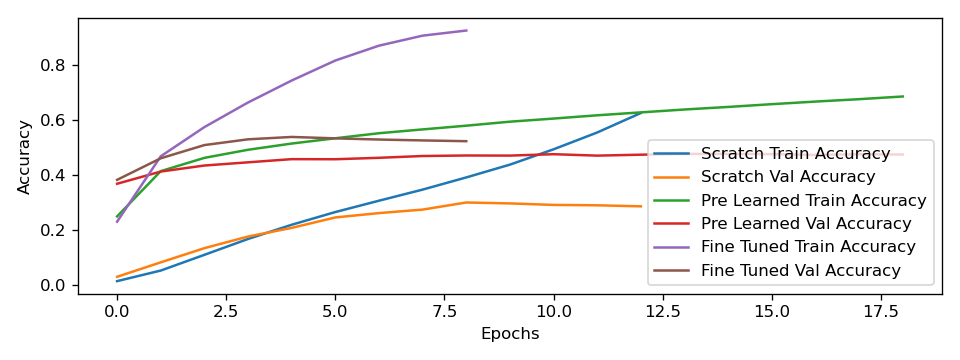
\includegraphics[width=1\linewidth]{/Part4.assets/task14.png}
        \caption{T4.1 Validation and Training Accuracy for Different Training Methods}\label{fig:t41}
        \vspace{-1cm}
    \end{center}
\end{figure}

% As can be seen from table~\ref{table:t41} and figure REF, using a pre trained model and freezing the weights results in a far smaller training time per epoch than training weights from scratch or fine tuning pre trained weights as expected. However, due to the pre training weights not being trained to this specific training freezing the weights results in a longer overall training time due to a greater number of epochs needed with still only a similar validation accuracy being achieved nto the model trained from scratch. This suggests that freezing the weights vs training from scratch is a worse strategy us perhaps unexpectedly it does not lead to lower training times and didn't in this case improve the test score. \\
% The use of a pre trained weights combined with fine tuning had a similar time per epoch as training from scratch but resulted in a better test accuracy. Although more epochs were used after the number of epochs at which the scratch training finished this method already had a higher validation accuracy suggesting it to be the superior training means in this case. 
% ADD REF TO A PAPER

As can be seen from table~\ref{table:t41} and figure~\ref{fig:t41}, using a pre-trained VGG-16 model and freezing the weights gave significantly worse performance than either training VGG-16 from scratch or fine tuning the weights. Despite having a faster training time per epoch even after twice the epochs as the other strategies the test, training and validation accuracy was roughly 8\% lower. This suggests perhaps that the features learned by the pre trained VGG image net model do not transfer well to the dataset used here. The features do work to an extent as it is still possible to get a relatively high test accuracy compared to training from scratch and is certainly better than untrained features. \\
There is little difference in the results between training the model from scratch or fine tuning the pre trained model which corroborates the idea that the pre-learned features don't transfer that well to this dataset. Interestingly, the fine tuned training accuracy is lower than that of training from scratch but the test and validation accuracy is marginally higher. This suggests that the features in the fine tuned model are more generalised and less over fit to the data. The result of this indicates that fine tuning the weights is better than starting from scratch but doesn't make a huge difference in this case. \\
The DenseNet121 model provided by Keras was used as the alternative model with its pre-trained weights being fine tuned to give the results shown in table~\ref{table:t41}. This model gave a better test accuracy with an increase of about a percent combined however, with a longer training time per epoch and greater inference time. The increased accuracy is expected as according to the keras website\cite{pretrained} DenseNet121 does have a higher score on the ImageNet challenge than VGG16. 
%https://keras.io/api/applications/
\\ The GPU used for all the results reported for this task is a Tesla P100-PCIE-16GB.

\section{Tutorial 5 Recurrent Neural Networks}

\paragraph{Task1: RNN Regression}
% - plot curves for different window sizes
% - discuss differences
\begin{figure}[ht]
    \begin{center}
        \includegraphics[width=1\linewidth]{/Part5.assets/t1.png}
        \caption{T5.1 Test predictions for different LSTM window sizes with a moving average filter and true values for reference}\label{fig:t51}
        \vspace{-0.7cm}
    \end{center}
\end{figure}
The plots in figure~\ref{fig:t51} show the predictions made for different LSTM window sizes. A common theme between all three of the plots shown is that despite the window size they all seem to lag slightly behind the actual dataset values, with this being especially noticeable at month 125. A reason for this could be that the value predicted is most correlated to the score from the last month giving a prediction close to this value. When training LSTM of different dimensions were tried as well as combing multiple LSTMs along with dense layers and dropout. No model tried was able to give a significant improvement as compared to the original model however meaning significant more complexity and epochs may be needed to achieve more accurate results.\\
%REF
As can be seen in the plot the greater the window size the more smoothed out the predictions tend to be with the effect looking similar to that of a moving average filter of size 16, a plot of which has been added for reference in figure~\ref{fig:t51}. This may indicate that the LSTM in weighting the effect of each input too evenly. 
%REF
% ADD PREDICTIONS GET BETTER
\paragraph{Task2: Text Embeddings}
% - table of test accuracy
% - appendix plots of val and train accuracy
% - discuss results
Table~\ref{table:t52} shows the test accuracy for the three different model types. As can be seen adding an LSTM and a larger embedding dimension made essentially no change to the test accuracy. Figures~\ref{fig:t521},\ref{fig:t522} and \ref{fig:t523} in the appendix show the training and validation accuracy curves. For the two methods that used an LSTM the validation accuracy settled almost immediately suggesting that it is difficult to get an accuracy much higher than the one achieved. When using the custom embedding the validation loss starts to increase over time indicating that overfitting occurs, a problem that is removed when using the glove embedding due to the glove embedding being more generalised. The use of the glove embedding did give an increase in accuracy which is expected as the embedding better represents the meaning of a word as opposed to being over fit to the training data in the custom embeddings. The lack of an LSTM gave the same score in the example sentences given, "the movie is boring and not good" for the negative score and "the movie is good and not boring" for the positive score. This is expected as the two sentences use the exact same words and so without a sense of order the model has no way of inferring the different sentiment. \\
The list of words most similar to "book" was generated for the two LSTM types. When using the Glove embedding the words generated were of a similar meaning or genre to "book", for instance "novel" and "author". The custom embedding, on the other hand, had no similarity in meaning, for example "points" and "stick". This is due to the fact that the glove embedding is trained in such a way as to give a similar embedding to words of a similar meaning and to allow combinations of words to give a summed embedding similar to words that have the same meaning as the words combined\cite{slides5}. This is not the case in the custom embedding, which is simply trained to try contain sentiment within the embedding.

%//TODO  ADD REFERENCE
\begin{table}[ht]
    \small
    \centering
    \begin{tabular}{|c|c|c|c|}
        \hline
        Model     & Test Accuracy & Neg. Score & Pos. Score \\
        \hline
        No LSTM & 85.24\%   & 0.368 & 0.368        \\
        LSTM  & 85.11\%  & 0.224 & 0.306         \\
        LSTM and Glove & 86.82\%   &   0.438 & 0.484     \\
        \hline
    \end{tabular}
    \medbreak
    \caption{T3.1 Test accuracy and score difference for different models}
    \vspace{-1cm}
    \label{table:t52}
\end{table}

\paragraph{Task3: Text Generation}

% - plot bleu against temp
% - discuss plot
% - discuss word generation differences (grammer etc)

\begin{figure}[ht]
    \begin{center}
        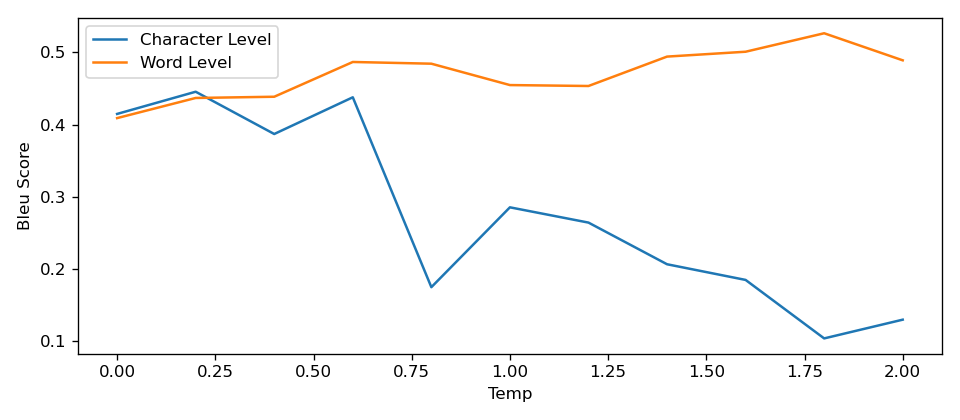
\includegraphics[width=1\linewidth]{/Part5.assets/t3.png}
        \caption{T5.1 Bleu score against temperature for character and word level models}\label{fig:t53}
        \vspace{-0.3cm}
    \end{center}
\end{figure}
% RE GENERATE GRAPH
Figure~\ref{fig:t53} shows how the bleu score is affected by temperature. For the character level model the trend is clearly that the bleu score decreases with a higher temperature, whilst for the word level model the blue score seems to increase slightly as temperature is increased. Since the bleu score does not take into account sentence meaning it is expected that in the case of the character level model an increased prevalence of words that don't exist gives a lower bleu score as the score is a measure of the number of matching words between the true text and the generated\cite{bleu}. Since the word level model doesn't give non existant words there is not much change in it's bleu score. 

When increasing the temperature the generated sentences changed significantly. The sentences generated with extremely low temperatures contained a lot of repetition but only real words were generated and the grammatical accuracy  and sentence meaning were not bad. As the temperature was increased so did the variation in the text along with the amount of incorrect words, accompanied with a decrease in overall sentence coherence. A temperature of about 1 gave the best combination of variation and accuracy for the character level model. For the word level model the problem of incorrect words is not present due to the words themselves being generated, meaning the change is only in variation and grammar. Since the grammar is bad for any temperature the change is not extremely noticeable and the decrease in repetition is the bigger change as the temperature is increased. The sentences generated do tend to make less sense the greater the temperature used to generate them.

\section{Tutorial 6 Representational Learning}

\paragraph{Task1: Non-linear Transformations}

% - accuracy mse (training and val) for no cnn, cnn and pca in table \\
% - describe two models \\
% - discuss results \\

Table~\ref*{table:t61} shows the results found for the three different encoding methods used. The final architecture of the autoencoders with no CNN was three dense layers with 256, 128 and 10 neurons respectively. The first two layers also employed RELU activation and the decoder architecture was the same as the encoding reversed. When using a CNN three different CNN layers were used with 128, 64 and 64 layers each and all CNN layers were of size 3x3. The CNN layers were followed by three dense layers of size 256,64 and 10. All layers used RELU activation apart from the last layer and the decoder used the same architecture in reverse. \\
As can be seen from table~\ref*{table:t61} the use of neural networks gave a large increase in accuracy as compared to PCA. The reason for the increased accuracy using neural nets is due to the ability to approximate non linear functions unlike linear PCA~\cite{pca}. The none CNN strategy has an optimal solution that is the same as a non linear PCA~\cite{pca}. Moving from a traditional NN to a CNN gave a small increase in performance in terms of accuracy although a fairly large decrease in MSE was found. This is expected as CNNs are better at extracting features from an image and so should be better at providing features for an encoding as compared to the traditional network.  

\begin{table}[ht]
    \small
    \centering
    \begin{tabular}{|c|c|c|c|}
        \hline
        Architecture     & Accuracy \% & MSE Train & MSE Val \\
        \hline
        No CNN & 91.67   & 0.0087 & 0.0089        \\
        CNN  & 96.09  & 0.0059 &   0.0068       \\
        PCA &  81.48  &  0.0258  &   0.0256   \\
        \hline
    \end{tabular}
    \medbreak
    \caption{T6.1 MSE and accuracy for different encoder architectures}
    \label{table:t61}
    \vspace{-0.8cm}
\end{table}

\paragraph{Task2: Custom Loss Functions}

Table~\ref{table:t62} shows how the MSE is dependent on the loss function used and figure~\ref*{fig:t62} shows the result filtering noise using a model trained with each loss function. The MS-SSIM and PSNR methods both give similar MSE and result in images that look very alike whereas the SSIM method gives an image that has fairly incorrect colours and gives a worse MSE. The SSIM function does give a similar level of noise removal in the image despite its colour inaccuracy. The increased performance of MS-SSIM vs SSIM is due to it working in a similar manner to SSIM by measuring structural similarity but operated at multiple scales giving a better metric\cite{ssim}. The degradation in colour seen with SSIM may be due to this metric not only valuing similar pixel values but also similar variance and cross correlation within a patch of pixels\cite{ssim}. The second two of which still give high scores if the overall average is shifted by a constant amount meaning a colour shift doesn't change two of these three metrics. PSNR may give a better MSE value due to its equations being directly related to MSE and so an improvement in PSNR gives an improvement in MSE\cite{psnr}. The better visual results in figure~\ref*{fig:t62} from MS-SSIM vs PSNR may be due to MS-SSIM judging similarity in a manner close to that of a human\cite{ssim}.
Some more information on the implementation of the loss functions can be found in the appendix \ref*{app:loss}.

\begin{table}[ht]
    \small
    \centering
    \begin{tabular}{|c|c|}
        \hline
        Loss Function & MSE Val \\
        \hline
        SSIM & 0.00781 \\
        MS-SSIM & 0.00562 \\
        PSNR & 0.00552 \\
        \hline
    \end{tabular}
    \medbreak
    \caption{T6.2 MSE for different loss functions}
    \label{table:t62}
    \vspace{-0.8cm}
\end{table}

\begin{figure}[ht]
    \begin{center}
        \includegraphics[width=1\linewidth]{/Part6.assets/task2.png}
        \caption{T5.1 Noisy Image, De-noised Image and Clean Image for different loss functions with SSIM resulting in bad colour accuracy and MS-SSIM giving the best result}\label{fig:t62}
        \vspace{-0.6cm}
    \end{center}
\end{figure}

% - report de-noised images for a few different models \\
% - report table to test mse for different models \\
% - discuss differences \\

\section{Tutorial 7 Variational Autoencoders}

\paragraph{Task 1: MNIST generation using VAE and GAN}

% - mse and inception score
% - mse and incep without KL divergance

As can be seen in table~\ref*{table:t71} The use of KL divergence in the variational autoencoder model gave a slightly higher MSE but a noticeable improvement in the Inception Score. The reduction in MSE is expected as without the KL divergence the loss is simply based on the difference between the generated image and the correct image thus optimising the model to reduce this value\cite{vae}. \\
If the distribution of the generated images is diverse in such a way that  images with a uniform spread of labels are generated i.e. $p(y)$ is uniform then a higher inception score is given\cite{kl-divergence} as this is the distribution of the true data. Since the KL divergence layer loss function tries to optimise to such a distribution\cite{kl-divergence} its presence helps to increase the inception score as is found in table~\ref*{table:t71}. \\
Table~\ref*{table:t71} shows that the cGAN network gave a higher Inception score than either of the VAE methods. Although a cGan does not rigorously learn the likelihood distribution unlike the VAE with KL it implicitly learns it through aiming to minimise the difference between $P(X)$ and $P(Z|Y)$\cite{gan}. In this case the GAN method has been more effective at creating accurate images and learning the distribution of images that the VAE methods, but this might not always be true.
% https://arxiv.org/pdf/1706.04987.pdf
% https://arxiv.org/pdf/1801.01973.pdf

\begin{table}[ht]
    \small
    \centering
    \begin{tabular}{|c|c|c|}
        \hline
        Model     & MSE & Inception \\
        \hline
        VAE KL & 0.0120 & 7.29 \\
        VAE No KL & 0.0110 & 5.95 \\
        GAN & na & 8.13 \\
        \hline
    \end{tabular}
    \medbreak
    \caption{T6.1 MSE and Inception scores with and without KL divergence as well as for the GAN model}
    \label{table:t71}
    \vspace{-0.7cm}
\end{table}

\paragraph{Task 2: Quantitative VS Qualitative Results}

Figure~\ref*{fig:t72} in the appendix shows several combinations of images with colour added by the MAE model and by the cGAN model approach compared to the real counterpart. The MAE found for the cGAN model was $0.0458$ and was $0.0449$ for the MAE trained model. In the images shown the cGAN approach appears to lead to more variation in colours within the image and more saturation. In the case of the MAE model the lower saturation may be due to the model trying to reduce the absolute error from the true image and so chooses colours that are closer to the average of all possible colours to try and minimise the error if it is wrong, resulting in the lower MAE score found. In the case of the cGAN the model is not trying to create the exact same colours as the true image but is instead trying to create colours with the same probability of occurring as the true colours\cite{gan}. This means it is able use a greater saturation without risking higher errors in the same way as the MAE model as the error is not directly related to the difference in value between the colour it produces and the true colour.

\section{Tutorial 8 Reinforcement Learning}

Figure~\ref*{fig:t81} shows the results found using SARSA and Q-Learning with $\epsilon$-greedy and softmax. The modification made are given in the appendix in section\ref*{app:modifications}.
\begin{figure}[ht]
    \begin{center}
        \includegraphics[width=1\linewidth]{/Part8.assets/t1.png}
        \caption{T5.1 Average Score of last 50 episodes for different RL techniques}\label{fig:t81}
    \end{center}
\end{figure}

\clearpage

{\small
    \bibliographystyle{ieee}
    \bibliography{egbib}
}

\section{Appendix}

\begin{figure}[ht]
    \begin{center}
        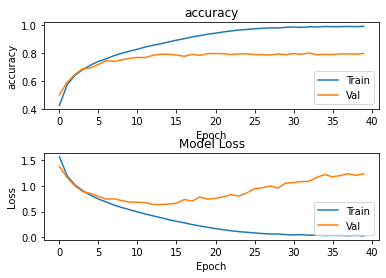
\includegraphics[width=1\linewidth]{/Part3.assets/task11.png}
        \caption{T2.1.1 Validation and Training Loss No Augmentation}\label{fig:t311}
    \end{center}
\end{figure}
\begin{figure}[ht]
    \begin{center}
        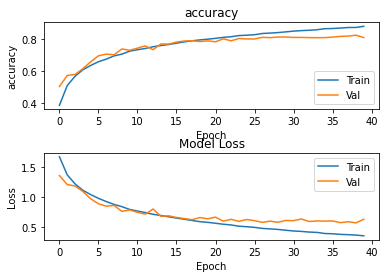
\includegraphics[width=1\linewidth]{/Part3.assets/task12.png}
        \caption{T2.1.1 Validation and Training Loss Soft Augmentation}\label{fig:t312}
    \end{center}
\end{figure}
\begin{figure}[ht]
    \begin{center}
        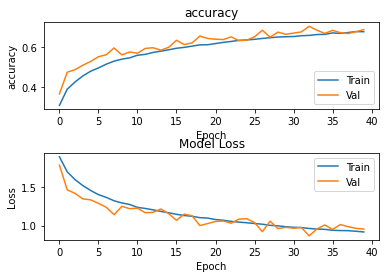
\includegraphics[width=1\linewidth]{/Part3.assets/task13.png}
        \caption{T2.1.1 Validation and Training Loss Hard Augmentation}\label{fig:t313}
    \end{center}
\end{figure}

\begin{figure}[ht]
    \begin{center}
        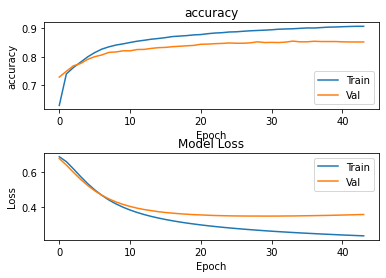
\includegraphics[width=1\linewidth]{/Part5.assets/task21.png}
        \caption{T2.1.1 Validation and Training Accuracy no LSTM}\label{fig:t521}
    \end{center}
\end{figure}
\begin{figure}[ht]
    \begin{center}
        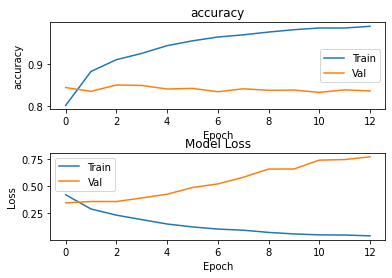
\includegraphics[width=1\linewidth]{/Part5.assets/task22.png}
        \caption{T2.1.1 Validation and Training Accuracy custom Embedding}\label{fig:t522}
    \end{center}
\end{figure}
\begin{figure}[ht]
    \begin{center}
        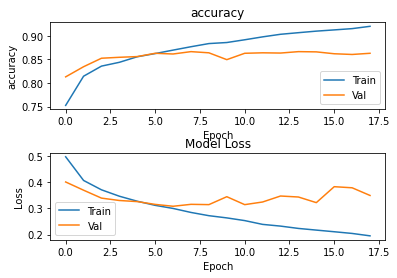
\includegraphics[width=1\linewidth]{/Part5.assets/task23.png}
        \caption{T2.1.1 Validation and Training Accuracy glove Embedding}\label{fig:t523}
    \end{center}
\end{figure}


\begin{figure}[ht]
    \begin{center}
        \includegraphics[width=1\linewidth]{/Part7.assets/task2.png}
        \caption{T7.2 }\label{fig:t72}
    \end{center}
\end{figure}

\FloatBarrier
\subsection{Custom Loss Function}\label{app:loss}
MS-SSIM and SSIM both give higher scores when two images are similar which was the opposite to what we want our loss functions to do. Thus $1-L$ (where L is the output of these functions) was taken as $1$ is the maximum score. It was found this method performed better than using $1/L$ in testing. In the case of PSNR $1/L$ was used as there is no limit on the value of PSNR with a higher value score being better. 

\subsection{DQNAgent Modifications}\label{app:modifications}
In order to implement softmax the "act" function had to be rewritten. The predicted scores for the two actions from the given state were found and then the softmax values of these scores were generated using teh given function. Finally a number between 0 and 1 was randomly generated. If this number was less than the first value given from the softmax output a 0 was returned otherwise a 1 was returned. \\
When implementing SARSA the score chosen for a given next state was no longer just the highest score given by the two available actions. Instead the action taken was chosen in the same way as act function, (either using epsilon greedy or softmax discussed above). The action chosen using either of the two methods was then used to choose which next score was taken.




\end{document}